\section{Basics of linear algebra} 
\begin{frame}\frametitle{Linear (in)dependence}
    A set of vectors $\{v_1, v_2,\cdots,v_n\}$ in a  vector space $\mathbb{V}$ is called \textbf{linearly independent} if
    the linear combination 
    \begin{equation*}
        \sum_{i=1}^n\alpha_iv_i=0
    \end{equation*}
    implies that $\alpha_1=\alpha_2=\cdots=\alpha_n=0$. If not, is called \textbf{linearly dependent}.  
\end{frame}

\begin{frame}\frametitle{Span and Basis}
    For a set of vectors $\{v_1, v_2,\cdots,v_n\}$ in a vector space $\mathbb{V}$, the set of linear combinations of 
    vectors in $\mathbb{V}$ is called the \textbf{span} of $\{v_1, v_2,\cdots,v_n\}$. i.e,
    \begin{equation*}
        \textbf{span}\{v_1, v_2,\cdots,v_n\} = \{\sum_{i=1}^n\alpha_iv_i|\forall\alpha_i\in\R{}, i=1, 2, \cdots,n\}
    \end{equation*}\\
    \vspace{10mm}
    A \textbf{basis} of a vector space $\mathbb{V}$ is an independent set of vectors that spans $\mathbb{V}$.
\end{frame}

\begin{frame}\frametitle{Matrix rank}
    Let $A\in\mathbb{R}^{d\times m}$ be a matrix, the \textbf{column rank} of $A$ is defined as the number of linearly independent columns,
    similar the \textbf{row rank} of $A$ is defined as the number of linear independent rows
    \vspace*{5mm}
    \begin{itemize}
        \item Row and column ranks are always the same for given matrix
        \item So we call it simply rank
    \end{itemize}
\end{frame}

\begin{frame}\frametitle{(vector)Subspace}
    Let $\mathbb{V}=(V,+,\cdot)$ be a vector space and $\emptyset\neq U\subseteq V$. Then $\mathbb{U}=(U,+,\cdot)$ is called vector \textbf{subspace} of $\mathbb{V}$
    if $\mathbb{U}$ is closed under $(+,\cdot)$ operations.
    \vspace*{10mm}
    \begin{itemize}
        \item $0\in\mathbb{V}$ always belongs to any subspaces  
        \item Lines and planes through the $0\in\R{3}$ are subspaces in $\R{3}$
        \item The intersection of arbitrarily many subspaces is a subspace itself
    \end{itemize}
\end{frame}

\begin{frame}\frametitle{Affine subspace}
    Let $\mathbb{V}$ be a vector space, $x \in \mathbb{V}$ and $\mathbb{U}\subseteq\mathbb{V}$ a subspace. Then the subset
    \begin{equation*}
        L = x + \mathbb{U} := \{x+u|\ u\in\mathbb{U}\}
    \end{equation*}
    is called \textbf{affine subspace} $\mathbb{V}$.
    \vspace*{5mm}
    \begin{itemize}
        \item An affine subspace excludes 0 if $x \notin \mathbb{U}$
        \item Points, lines and planes are affine subspaces in $\R{3}$
        \item In $\R{d}$, the (d-1)-dimensional affine subspaces are called hyperplanes.
    \end{itemize}
\end{frame}


\begin{frame}\frametitle{Dot / Inner product}
    A \textbf{dot product} of $x=(x_1,x_2,\cdots,x_d), y=(y_1,y_2,\cdots,y_d) \in\R{d}$ is defined as
    \begin{equation*}
        x\boldsymbol{\cdot}y = \sum_{i=1}^dx_iy_i
    \end{equation*}\\

    \pause An \textbf{inner product} of a real scalar vector space $\mathbb{V}$ is a function of vector pairs $x,y\in\mathbb{V}$,  which is denoted by $\langle x,y\rangle$ and
    satisfies the following three properties:
    \begin{itemize}
        \item (commutativity) $\langle x,y\rangle = \langle y,x\rangle$ for any $x,y\in\mathbb{V}$.
        \item (linearity) $\langle \alpha x+\beta y, z\rangle = \alpha\langle x, z\rangle + \beta\langle y, z\rangle$ \\for any $\alpha,\beta \in\R{}$ and $x,y,z \in\mathbb{V}$.
        \item (positive definiteness) $\langle x,x \rangle \geq 0$ for any $x \in\mathbb{V}$ and $\langle x,x \rangle =0$ if and only if $x = 0$.
    \end{itemize}
    \vspace*{3mm}
    \pause\begin{itemize}
        \setlength{\itemindent}{-1em}
        \item A dot product is an inner product but the reverse is not true
        \item For $x=(x_1, x_2), y=(y_1, y_2)$, operation $\langle x,y \rangle=x_1y_1+2x_2y_2$ is also an inner product 
      \end{itemize}    
\end{frame}

\begin{frame}\frametitle{Outer product}
    The outer product is operation between two vectors $x\in\R{d},y\in\R{m}$ defined as
    \begin{equation*}
        x\otimes y = xy^T\in\mathbb{R}^{d\times m}
    \end{equation*}
    \begin{itemize}
        \item Rank of outer product of two vectors is 1
    \end{itemize}
\end{frame}

\begin{frame}\frametitle{Norms}
    A norm $||\cdot||$ on a vector space $\mathbb{V}$ is a function $||\cdot|| : \mathbb{V}\to\R{}$ satisfying the following properties:
    \vspace*{6mm}
    \begin{itemize}
        \item (nonnegativity) $||x||\geq0$ for any $x\in \mathbb{V}$ and $||x||=0$ if and only if $x=0$
        \item (positive homogeneity) $||\alpha x|| = |\alpha|\cdot||x||$ for any $x\in\mathbb{V}$ and $\alpha\in\R{}$.
        \item (triangle inequality) $||x + y||\leq||x|| + ||y||$ for any $x, y \in \mathbb{V}$
    \end{itemize}
\end{frame}

\begin{frame}\frametitle{$\ell_p$ Norms}
    For a $p\geq 1$, the $\ell_p$-norm on $\R{d}$ is given by the formula
    \begin{equation*}
        ||x||_p = \sqrt[p]{\sum_{i=1}^d|x_i|^p}
    \end{equation*}\\
    \vspace{10mm}
    For a $p=\infty$, the $\ell_\infty$-norm on $\R{d}$ is given by
    \begin{equation*}
        ||x||_\infty = \max_{i=1,2,\cdots,d}|x_i|
    \end{equation*}
\end{frame}

\begin{frame}\frametitle{$\ell_p$ Norms}
    For a $p=0$, the $\ell_0$-norm on $\R{d}$ is given by
    \begin{equation*}
        \|x\|_0 = \#\text{ of non zero components} 
    \end{equation*}
    \begin{itemize}
        \item e.g) $x=(2,0,3), \|x\|_0=2$
        \item This assumes $0^0=1$
        \item In fact, $\ell_0$ norm is not a norm. Because it doesn't satisfy the positive homogeneity
    \end{itemize}
\end{frame}

\begin{frame}\frametitle{Induced norm}
    Any inner product induces a norm, defined as
    \begin{equation*}
        ||x||:=\sqrt{\langle x,x\rangle}
    \end{equation*}
    which is called \textbf{induced norm} by the given inner product $\langle\cdot,\cdot\rangle$\\
    \vspace*{10mm}
    \begin{itemize}
        \item Induced norms satisfy the properties of norms
        \item $\ell_2$ norm is induced norm by dot product
        \item Not all the norms are induced norm, e.g, $\ell_1$-norm
    \end{itemize}
\end{frame}

\begin{frame}\frametitle{Angle}
    An \textbf{angle} $\omega$ of two vectors $x,y\in\mathbb{V}$ equipped with $ \langle \cdot, \cdot \rangle$ is defined by
    \begin{equation*}
        \omega = \frac{\langle x,y\rangle}{||x||\ ||y||} 
    \end{equation*}
    where the $||\cdot||$ is induced norm
    \vspace*{10mm}
    \begin{itemize}
        \item $-1\leq\omega \leq 1 $
        \item The two vectors have different angles depending on which inner product is used
        \item $arccos(w)$ is an angle of two vectors in radian
    \end{itemize}
\end{frame}

\begin{frame}\frametitle{Cauchy–Schwarz inequality}
    For vector space $\mathbb{V}$, an inner product $\langle \cdot,\cdot \rangle$ and its induced norm $||\cdot ||$ satisfies the \textbf{Cauchy-Schwarz inequality}
    \begin{equation*}
        |\langle x,y\rangle|\leq ||x||\ ||y||
    \end{equation*}
\end{frame}

\begin{frame}\frametitle{Hölder inequality}
    For vector space $\mathbb{V}$ and $p,q\in[1,\infty]$ satisfying $\frac{1}{p}+\frac{1}{q}=1$, the
    $||\cdot||_p, ||\cdot||_q$ satisfy the \textbf{Hölder inequality}
    \begin{equation*}
        x\boldsymbol{\cdot}y\leq ||x||_p\ ||y||_q
    \end{equation*}
    \vspace*{5mm}
    \begin{itemize}
        \item The pair $(p,q)$ are called Hölder conjugates of each other
        \item Cauchy–Schwarz inequality is the case of $p=q=2$
    \end{itemize}
\end{frame}

\begin{frame}\frametitle{Minkowski inequality}
    For vector space $\mathbb{V}$ and $p\in[1,\infty]$, the
    $||\cdot||_p$ satisfies the \textbf{Minkowski inequality}
    \begin{equation*}
        ||x+y||_p\leq ||x||_p+||y||_p
    \end{equation*}
    \vspace*{5mm}
    \begin{itemize}
        \item From this inequality, $\ell_p$-norms satisfy the triangle inequality property
    \end{itemize}
\end{frame}

\begin{frame}\frametitle{Young's inequality}
    For $a,b\geq 0$ and $p,q>1$ s.t $\frac{1}{p}+\frac{1}{q}=1$, the \textbf{Young's inequality} is as follows
    \begin{equation*}
        ab\leq\frac{a^p}{p}+\frac{b^q}{q}
    \end{equation*}
    Equality holds if and only if $a^p=b^q$
\end{frame}

\begin{frame}\frametitle{Eigenvalues and eigenvectors}
    Let $A\in\mathbb{R}^{d\times d}$ be a square matrix. Then $\lambda\in\R{}$ is an \textbf{eigenvalue} of $A$ and $x\in\R{d}/\{0\}$
    is the corresponding \textbf{eigenvector} of $A$ if
    \begin{equation*}
       Ax=\lambda x
    \end{equation*}
    \vspace*{2mm}
    \begin{itemize}
        \item There are at most d eigenvalues(and corresponding eigenvectors)
        \item For any symmetric (real)matrix $A$, all its eigenvalues are real
        \item All eigenvectors of a symmetric (real)matrix are orthogonal to each other
    \end{itemize}
\end{frame}

\begin{frame}\frametitle{Eigenspace and Eigenspectrum}
    The set of all eigenvectors of $A$ associated with an eigenvalue $\lambda$ spans a subspace of $\R{d}$,
    which is called the \textbf{eigenspace} of $A$ with respect to $\lambda$ and is denoted by $E_\lambda$\\
    \vspace*{10mm}
    The span of all the eigenvectors of $A$ is called the \textbf{eigenspectrum} of $A$
\end{frame}

\begin{frame}\frametitle{Positive (semi)definite matrices}
    The given square matrix $A\in\mathbb{R}^{d\times d}$ is called \textbf{positive semidefinite}, if for any $x\in\R{d}$
    \begin{equation*}
        x^TAx\geq0
    \end{equation*}
    when the inequality holds strictly, the matrix called \textbf{positve definite}
    \vspace*{10mm}
    \begin{itemize}
        \item  For any matrix $A$, $A^TA$ is symmetric and positive semidefinite
        \item  For any square matrix $A$,\\ positive definiteness(respectively, semidefiniteness) $\Longleftrightarrow$ \\every eigenvalues of $A$ are positive (respectively, nonnegative)
        
    \end{itemize}
\end{frame}

\begin{frame}\frametitle{Matrix Norms}
    Frobenius norm is norm of any $m\times n$ matrix A defined as square root of component wise squared sum 
    \begin{equation*}
        \|A\|_F \equiv \sqrt{\sum_{i=1}^m \sum_{j=1}^n\left|a_{i j}\right|^2} 
    \end{equation*}
    \begin{itemize}
        \item $\|A\|_F = \sqrt{Tr(AA^T)}$
    \end{itemize}
\end{frame}

\begin{frame}\frametitle{Matrix Norms}
    Vector $\ell_p$ norm induced matrix $\ell_p$ norm is norm of any $m\times n$ matrix A defined as 
    \begin{equation*}
        \|A\|_p=\sup _{x \neq 0} \frac{\|A x\|_p}{\|x\|_p}
    \end{equation*}
    \begin{itemize}
        \item Matrix $\ell_1$ norm is the maximum absolute column sum of the matrix
        \item Matrix $\ell_\infty$ norm is the maximum absolute row sum of the matrix
    \end{itemize}
\end{frame}

\begin{frame}\frametitle{Matrix Norms}
    \begin{itemize}
        \item For example, for
        $A=\left[\begin{array}{ccc}
        -3 & 5 & 7 \\
        2 & 6 & 4 \\
        0 & 2 & 8
        \end{array}\right]
        $
        we have that
        $$
        \begin{aligned}
        & \|A\|_1=\max (|-3|+2+0 ; 5+6+2 ; 7+4+8)=\max (5,13,19)=19 \\
        & \|A\|_{\infty}=\max (|-3|+5+7 ; 2+6+4 ; 0+2+8)=\max (15,12,10)=15
        \end{aligned}
        $$
        \item Matrix $\ell_2$ norm, also called spectral norm, is the largest singular value of $A$ $$\|A\|_2=\sqrt{\lambda_{\max }\left(A^T A\right)}=\sigma_{\max }(A)$$
        \item $\|A\|_2^2=\|A^TA\|_2=\|AA^T\|_2$
        \item $\|A\|_2\leq\|A\|_F$
    \end{itemize}
\end{frame}

\section{Basics of multivariable calculus}

\begin{frame}\frametitle{Gradient}
    For a differentiable function $f:\R{d}\to\R, x\in\R{d}$ and $x=(x_1,x_2,\cdots,x_d)$, the collection of partial derivatives 
    is called the \textbf{gradient} of $f$ defined as
    \begin{align*}
        \nabla_xf=grad\ f=\frac{df}{dx}&= \begin{bmatrix}
            \frac{\partial f}{\partial x_1} \\
            \frac{\partial f}{\partial x_2} \\
               \vdots \\
               \frac{\partial f}{\partial x_d}
             \end{bmatrix}\in\R{d}
      \end{align*}
      \begin{itemize}
        \item It has the steepest ascending direction infinitesimally, similarly the opposite is the steepest descending direction.
      \end{itemize}    
\end{frame}

\begin{frame}\frametitle{Hessian}
    For a twice continuously differentiable function $f:\R{d}\to\R,\ x\in\R{d}$ and $x=(x_1,x_2,\cdots,x_d)$, the collection of second-order partial derivatives
    is called the \textbf{Hessian} of $f$ defined as
    \begin{align*}
        \nabla_x^2f=H\ f=\frac{d^2f}{dx^2}&= \begin{bmatrix}
            \frac{\partial^2 f}{\partial x_1^2} & \frac{\partial^2 f}{\partial x_2 \partial x_1} &\cdots & \frac{\partial^2 f}{\partial x_d \partial x_1} \\
            \frac{\partial^2 f}{\partial x_1\partial x_2} & \frac{\partial^2 f}{\partial x_2^2} &\cdots & \frac{\partial^2 f}{\partial x_d \partial x_2} \\
            \vdots&\vdots&\cdots&\vdots \\
            \frac{\partial^2 f}{\partial x_1\partial x_d} & \frac{\partial^2 f}{\partial x_2\partial x_d} &\cdots & \frac{\partial^2 f}{\partial x_d^2} \\
             \end{bmatrix}\in\mathbb{R}^{d\times d}
      \end{align*}
      \begin{itemize}
        \item If the above function is twice continuously differentiable, the Hessian matrix is always a real symmetric matrix
        \item The eigenvectors and eigenvalues of Hessian is directly related to curvature of the given function
      \end{itemize}      
\end{frame}



\section{Convex Sets}
\subsection{Definition and Examples}
\begin{frame}\frametitle{Convex Sets: Definition}
    \begin{definition}
     A set $C \subseteq \mathbb{R}^n$ is \textbf{convex} if 
    \begin{equation*}
        \forall x_1, x_2 \in C, \forall \lambda \in [0,1] \Rightarrow \lambda x_1 + (1 - \lambda) x_2 \in C
    \end{equation*}
    \end{definition}

    \hspace{10mm}
    \begin{figure}
    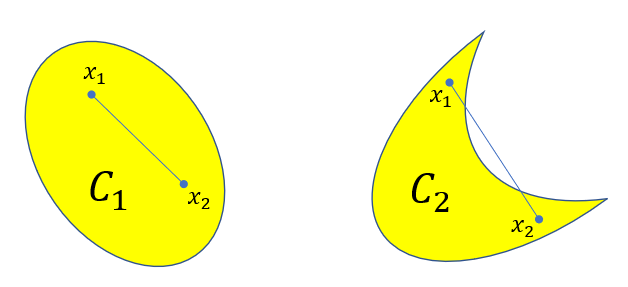
\includegraphics[scale=0.5]{./figures/convex_nonconvex_examples.png}
    \caption{Examples of convex and non-convex sets}
    \end{figure}
\end{frame}

\begin{frame}\frametitle{Examples of Convex Sets}
    \begin{itemize}
        \item \textbf{Simplex}: A simplex $\{x \in \mathbb{R}^n \mid \sum_{i=1}^{n} x_i = 1 \text{ and for all } i=1,2, ... , n, x_i \geq 0\}$ in $\mathbb{R}^n$ is a convex set.
        For any $x,y$ in the simplex, and $\lambda \in [0,1]$,
        \begin{equation*}
            \sum_{i=1}^{n} (\lambda x + (1-\lambda) y)_i = \lambda \sum_{i=1}^{n} x_i + (1-\lambda) \sum_{i=1}^{n} y_i = 1
        \end{equation*}
        and each element of $\lambda x + (1-\lambda) y$ is still non-negative.
        \item \textbf{Set of psd matrices}: A set of $n \times n$ positive semidefinite (psd) matrices, denoted by $S_{+}^{n}$, is convex. 
        Take $M_1, M_2 \in S_{+}^{n}$. Then for all $x \in \mathbb{R}^n, \lambda \in [0,1]$,
        \begin{equation*}
            x^T (\lambda M_1 + (1-\lambda) M_2) x = \lambda (x^T M_1 x) + (1-\lambda) (x^T M_2 x) \geq 0
        \end{equation*}
        So $\lambda M_1 + (1-\lambda) M_2 \in S_{+}^{n}$.
        \item \textbf{Set of copositive matrices}: An $n \times n$ matrix $M$ is copositive if $x^T M x \geq 0$ for any $x \in \mathbb{R}_{+}^{n}$. 
        We can show in the same way as above that the set of copositive matrices is a convex set. Note that since a psd matrix is always copositive, 
        the set of psd matrices is included in the set of copositive matrices.
    \end{itemize}
\end{frame}

\subsection{Hyperplane}
\begin{frame}\frametitle{Hyperplane and Half-spaces}
    \begin{definition}
        In $\mathbb{R}^{n}$, given some $s \in \mathbb{R}^{n}$ and $b \in \mathbb{R}$, we define a \textbf{hyperplane} as
        \begin{equation*}
            H_{s,b} = \{x \in \mathbb{R}^{n} \mid  s^{T} x = b\}
        \end{equation*}
        Here, $s$ is called the \textbf{normal vector} of $H_{s,b}$.\\
        Moreover, a hyperplane $H_{s,b}$ divides $\mathbb{R}^n$ into two \textbf{half-spaces}
        \begin{equation*}
            H_{s,b}^{-} = \{x \in \mathbb{R}^n \mid  s^T x \leq b\}, \hspace{2mm} H_{s,b}^{+} = \{x \in \mathbb{R}^n \mid  s^T x \geq b\}
        \end{equation*}
    \end{definition}

    \begin{figure}
    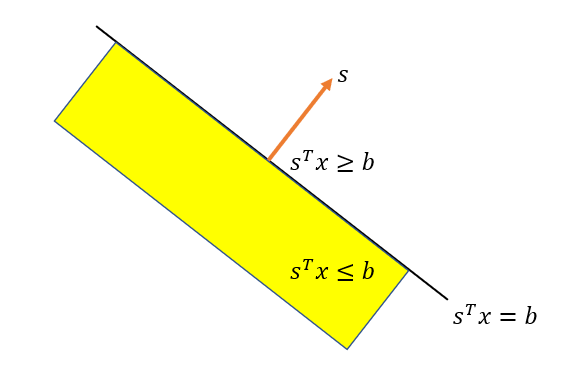
\includegraphics[scale=0.25]{./figures/hyperplane_halfspaces.png}
    \caption{Hyperplane with normal vector, two half-spaces}
    \end{figure}
\end{frame}

\begin{frame}\frametitle{Hyperplane and Convexity}
    A convex set can be "carved out" from half-spaces. 
    Formally, a closed convex set is the intersection of every closed half-spaces that contain the set. This property is equivalent to the separating hyperplane theorem.\\
    \begin{theorem}
        \textbf{Separating hyperplane theorem}: Let $\mathcal{X} \subset \mathbb{R}^n$ be a closed convex set, and $x_0 \in \mathbb{R}^n \setminus \mathcal{X}$.
        Then, there exists $w \in \mathbb{R}^n$ and $t \in \mathbb{R}$ such that
        \begin{equation*}
            \langle w, x_0 \rangle < t, \text{ and } \forall x \in \mathcal{X}, \langle w, x \rangle \geq t
        \end{equation*}
    \end{theorem}

    \begin{figure}
    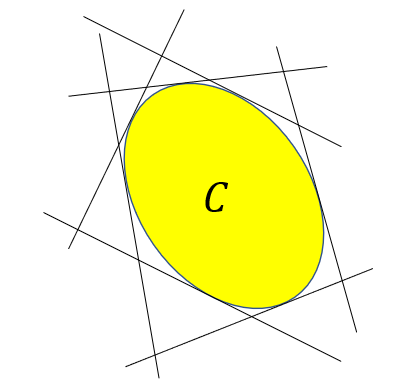
\includegraphics[scale=0.25]{./figures/carving_convex_set.png}
    \caption{Convex Set can be seen as intersection of half-spaces}
    \end{figure}
    
\end{frame}

\begin{frame}\frametitle{Example of Separating Hyperplanes}

    Separating hyperplane between the set of psd matrices and a symmetric matrix $\hat{M}$ that is not psd.\\
    Since $\hat{M}$ is symmetric, it has the eigenvalue decomposition $\hat{M} = \sum_{i} \hat{\lambda}_i \hat{v}_{i} \hat{v}_{i}^{T}$,
    where the eigenvectors are orthonormal.
    Since it is not psd, there is $i \in \{1,2, ... ,n\} $ such that $\hat{\lambda}_i < 0$.
    For simplicity, assume that $i = 1$. Now let $s = \hat{v}_1 \hat{v}_{1}^{T}$ and $b=0$.
    Then, we have
    \begin{align*}
        \langle s, \hat{M} \rangle ={ }& \langle \hat{v}_1 \hat{v}_{1}^{T} , \hat{M} \rangle = tr(\hat{M}\hat{v}_{1} \hat{v}_{1}^{T}) \\
        ={ }& tr(\hat{v}_{1}^{T} M \hat{v}_{1})\\
        ={ }& \hat{v}_{1}^{T} \hat{M} \hat{v}_{1}\\
        ={ }& \hat{v}_{1}^{T} (\sum_{i} \hat{\lambda}_i \hat{v}_{i} \hat{v}_{i}^{T}) \hat{v}_{1} = \hat{v}_{1}^{T} (\hat{\lambda}_1 \hat{v}_{1}) = \hat{\lambda}_1 < 0
    \end{align*}
    This implies that $\hat{M} \in H_{s,b}^{-}$.\\
    For any $M \in S_{+}^{n}$, $\langle s, M \rangle = \langle \hat{v}_1 \hat{v}_{1}^{T} , M \rangle = \hat{v}_{1}^{T} M \hat{v}_{1} \geq 0$ since $M$ is psd.
    So, $S_{+}^{n} \subseteq H_{s,b}^{+}$, and $H_{s,b}$ is the separating hyperplane.
\end{frame}

\subsection{Cones}
\begin{frame}\frametitle{Cones and Polar Cones}
    \begin{definition}
        A set $K$ is called a \textbf{cone} if
        \begin{equation*}
            \forall x_1, x_2 \in K, \forall \alpha_1, \alpha_2 \geq 0 \Rightarrow \alpha_1 x_1 + \alpha_2 x_2 \in K
        \end{equation*}
        Given a cone $K$, a \textbf{polar cone} of $K$, $K^{o}$ is also a cone defined as
        \begin{equation*}
            K^{o} = \{z \mid \langle z, x \rangle \leq 0, \forall x \in K\}
        \end{equation*}
    \end{definition}

    \textbf{Note}. A cone is always convex. Any subspace is a cone, but not vice versa.

    \begin{figure}
    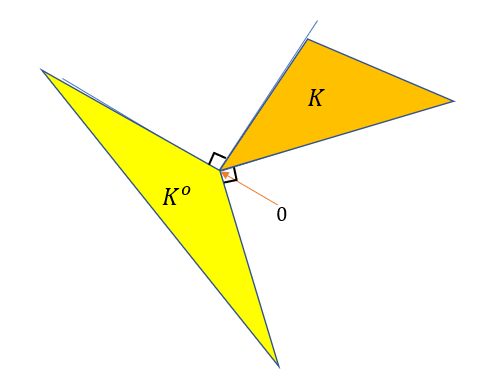
\includegraphics[scale=0.25]{./figures/cone_polarcone.png}
    \caption{A cone and its polar cone}
    \end{figure}
\end{frame}

%% insert picture of tangent cone and normal cone for each points
\begin{frame}\frametitle{Tangent Cones and Normal cones}
    \begin{definition}
        Given a set $\mathfrak{X}$ and a point $x \in \mathfrak{X}$, a \textbf{tangent cone} of $\mathfrak{X}$ at $x$, denoted as $T_\mathfrak{X}(x)$,
        is informally the set of directions $x$ can move inside $\mathfrak{X}$.
    \end{definition}

    \begin{definition}
        A \textbf{normal cone} of $\mathfrak{X}$ at $x$, denoted as $N_\mathfrak{X}(x)$, is a polar cone of the tangent cone of $\mathfrak{X}$ at $x$.
    \end{definition}


\end{frame}

\begin{frame}\frametitle{Tangent Cones and Normal Cones}
    \begin{itemize}
        \item If $x$ is an interior point of $\mathfrak{X}$, then $T_\mathfrak{X}(x) = \mathbb{R}^n$ and $N_\mathfrak{X}(x)=\{0\}$.
        \item If $x$ is a "smooth" boundary point, then $T_\mathfrak{X}(x)$ is the half-space including $\mathfrak{X}$ and $N_\mathfrak{X}(x)=\{s\}$ where the half-space and normal vector $s$ are from the supporting hyperplane $H_{s,b}$ of $\mathfrak{X}$ at $x$.
        \item If $x$ is a "non-smooth" boundary point of $\mathfrak{X}$, then $T_\mathfrak{X}(x)$ and $N_\mathfrak{X}(x)$ are shown below.
    \end{itemize}

    \begin{figure}
    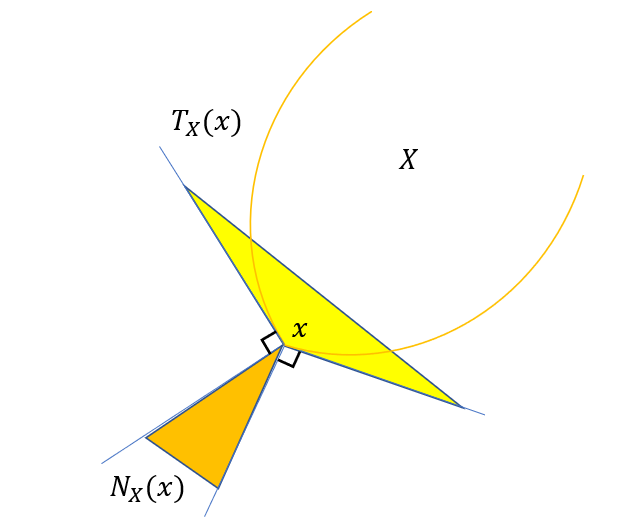
\includegraphics[scale=0.3]{./figures/tangent_cone.png}
    \caption{A tangent cone and its normal cone at non-smooth boundary point}
    \end{figure}
\end{frame}


%%%%%%%%%%%%%%%%%%%%%%%%%%%%%%%%%%%%%%%%%%%%%%%%%%%%%%%%%
\section{Convex Functions}

\subsection{Definitions}
\begin{frame}\frametitle{Convex Functions: Definitions}
    \begin{definition}
        A function $f: \mathbb{R}^n \rightarrow \mathbb{R}$ is convex if
        \begin{equation*}
            \forall x, y \in \mathbb{R}^n, \forall \lambda \in [0,1] \Rightarrow f(\lambda x + (1-\lambda)y) \leq \lambda f(x) + (1-\lambda)f(y)
        \end{equation*}
    \end{definition}

    \begin{definition}
        Suppose a function $f: \mathbb{R}^n \rightarrow \mathbb{R}$ is differentiable. Then it is convex if given any $x \in \mathbb{R}^n$,
        \begin{equation*}
            f(y) \geq f(x)+ \langle \nabla f(x), y-x \rangle \hspace{1mm} \text{for all} \hspace{1mm} y \in \mathbb{R}^n
        \end{equation*}
    \end{definition}
    \begin{definition}
        Suppose a function $f: \mathbb{R}^n \rightarrow \mathbb{R}$ is twice differentiable. Then it is convex if for any $x \in \mathbb{R}^n$, the Hessian $\nabla f^2 (x)$ is positive semidefinite.
    \end{definition}
    
\end{frame}

\begin{frame}\frametitle{Example: Quadratic Function}
    We will show that the quadratic function
     $f:\mathbb{R}^n \rightarrow \mathbb{R}$ defined by $f(x) = x^T Q x$ where $Q \succcurlyeq 0$, is convex using the three definitions.\\
    \textbf{Definition 1}: 
    \begin{equation*}
        \{\lambda f(x) + (1-\lambda)f(y)\} -  f(\lambda x + (1-\lambda)y) = (\lambda - \lambda^2)(y-x)^T Q (y-x) \geq 0 
    \end{equation*}
    
    \textbf{Definition 2}: $\nabla f(x) = 2Qx$. Then
    \begin{equation*}
        f(y) - \{f(x)+\langle \nabla f(x), y-x \rangle\} 
        = (y-x)^{T}Q(y-x) \geq 0
    \end{equation*}
    for all $y \in \mathbb{R}^n$.

    \textbf{Definition 3}: $\nabla^2 f(x) = 2Q \succcurlyeq 0$.
    
\end{frame}

\begin{frame}\frametitle{Example: Maximum of Convex Function}
    The maximum function of convex functions is convex. This can be shown from Definition 1.
    \begin{itemize}
        \item A function returning the largest element: 
        A function $f:\mathbb{R}^n \rightarrow \mathbb{R}$ defined as $f(x) = f(x_1, x_2, ... , x_n) = max(x_1, x_2, ... , x_n) = max(e_1^T x, e_2^T x, ... , e_n^T x)$ 
        is convex since each $e_i^T x$ is linear and hence convex.
        \item Maximum eigenvalue of symmetric matrix: For a symmetric matrix $Q$, $f(Q) = \lambda_{max} (Q)$. 
        We show that $f$ is convex. Recall that if $Q$ is symmetric, 
        then $x^{T}Qx \leq \lambda_{max} ||x||_2^2$ and the equality holds when $x$ is the eigenvector corresponding to $\lambda_{max}$. 
        So $\lambda_{max} = \text{sup}\hspace{1mm} x^T Qx$ subject to $||x||_2 = 1$, and since each $x^T Qx$ is a linear function of $Q$, 
        (observe that $x^T Qx = \langle x x^T, Q \rangle $), $f$ is a convex function.
    \end{itemize}
\end{frame}

\begin{frame}\frametitle{Subgradients and Subdifferentials}
    The second definition of convex functions can be extended to non-differentiable convex functions.
    \begin{definition}
        Given a function $f: \mathbb{R}^n \rightarrow \mathbb{R}$, it is convex if given any $x \in \mathbb{R}^n$, there exists $g \in \mathbb{R}^n$ such that
        \begin{equation*}
            f(y) \geq f(x)+ \langle g, y-x \rangle \hspace{1mm} \text{for all} \hspace{1mm} y \in \mathbb{R}^n
        \end{equation*}
    \end{definition}

    Note that if $f$ is convex and differentiable, $g=\nabla f(x)$ is unique $g$ that satisfy the above inequality.\\
    \begin{definition}
        For a convex function $f: \mathbb{R}^n \rightarrow \mathbb{R}$ and a point $x \in \mathbb{R}^n$, 
        a vector $g \in \mathbb{R}^n$ such that $ f(y) \geq f(x)+ \langle g, y-x \rangle \hspace{1mm} \text{for all} \hspace{1mm} y \in \mathbb{R}^n$ is called a \textbf{subgradient} at $x$. 
        A set of subgradients at $x$ is called the \textbf{subdifferential} of $f$ at $x$ and is denoted as $\partial f(x)$.
    \end{definition}
\end{frame}

\subsection{Monotone Property of Gradient}
\begin{frame}\frametitle{Monotone Property of Gradient}
    \begin{theorem}
        $f$ is convex according to Definition 2 if and only if it's gradient has the monotone property, that is, $\langle \nabla f(x) - \nabla f(y), x-y \rangle \geq 0$.
    \end{theorem}
    \begin{proof}
        First, assume that $f$ is convex according to Definition 2.\\
        (i) Then, by Definition 2, we have two inequalities 
        \begin{equation*}
            f(y) \geq f(x) + \langle \nabla f(x), y-x \rangle,\text{ } f(x) \geq f(y) + \langle \nabla f(y), x-y \rangle
        \end{equation*}
        for all $x, y \in \mathbb{R}^n$.
        Adding them gives $0 \geq \langle \nabla f(x) - \nabla f(y), y-x \rangle$.\\
    \end{proof}
\end{frame}

\begin{frame}\frametitle{Monotone Property of Gradient}
    \begin{proof}
        Now assume that $\nabla f$ has the monotone property. \\
        (ii) Define a function $g:[0,1] \rightarrow \mathbb{R}$ as $g(t)=f(tx+(1-t)y)=f(y+t(x-y))$. 
        Its gradient is given as $g'(t) = [\nabla f(y+t(x-y))]^T (x-y) = \langle \nabla f(y+t(x-y)), x-y \rangle$. 
        By the Fundamental Theorem of Calculus, we have
        \begin{equation*}
            \int_{0}^{1} g'(t)dt = g(1) - g(0) = f(x) - f(y) \text{ or } f(x) = f(y) + \int_{0}^{1} g'(t) dt
        \end{equation*}
        (iii) We claim $g'(t)$ is minimized at $t=0$.
        By the monotone property,
        \begin{align*}
            { }&\langle \nabla f(y+t(x-y)) - \nabla f(y) , y+t(x-y) - y \rangle\\
            ={ }& \langle \nabla f(y+t(x-y)), t(x-y) \rangle - \langle \nabla f(y), t(x-y) \rangle\\
            ={ }& t(g'(t) - g'(0)) \geq 0
        \end{align*}
    \end{proof}
\end{frame}

\begin{frame}\frametitle{Monotone Property of Gradient}
    \begin{proof}
        Therefore, $g'(t)$ has its minimum at $t=0$.
        (iv) From the results of (ii) and (iii),
        \begin{align*}
            f(x) ={ }& f(y)+\int_{0}^{1} g'(t)dt\\
            \geq{ }& f(y) + \int_{0}^{1} g'(0)dt\\
            ={ }& f(y) + g'(0)\\
            ={ }& f(y) + \langle \nabla f(y), x-y \rangle
        \end{align*}
        and $f$ is convex according to Definition 2.
    \end{proof}
\end{frame}


\section{Optimality Conditions for Convex Problems}
\subsection{Optimality Conditions}
\begin{frame}\frametitle{Optimality Condition for Smooth, Unconstrained Problem}
    \hspace{2mm}Consider the problem \textbf{$\text{min} \hspace{1mm} f(x)$} where $f: \mathbb{R}^n \rightarrow \mathbb{R}$ is convex and differentiable.\\
    \vspace*{3mm}
    \begin{theorem}
        $\hat{x}$ is an optimal solution to the above problem if and only if $\nabla f(\hat{x}) = 0$.
    \end{theorem}
    \begin{proof}
        Only prove the "if" part. Apply Definition 2 for convex functions to point $\hat{x}$. Then for all $y \in \mathbb{R}^n$, $f(y) \geq f(\hat{x}) + \langle \nabla f(\hat{x}), y-\hat{x} \rangle = f(\hat{x})$ for all $y \in \mathbb{R}^n$. So, $\hat{x}$ minimizes $f$.\\
    \end{proof}
\end{frame}

\begin{frame}\frametitle{Optimality Condition for Unconstrained Problem}
    \hspace{2mm}Now consider the problem \textbf{$\text{min} \hspace{1mm} f(x)$} where $f: \mathbb{R}^n \rightarrow \mathbb{R}$ is convex and not necessarily differentiable.\\
    \vspace*{3mm}
    \begin{theorem}
        $\hat{x}$ is an optimal solution to the above problem if and only if $0 \in \partial f(\hat{x})$.
    \end{theorem}
    \begin{proof}
        Only prove the "if" part. Apply definition of subgradients to function $f$ at point $\hat{x}$. Then for all $y \in \mathbb{R}^n$, $f(y) \geq f(\hat{x}) + \langle 0, y-\hat{x} \rangle = f(\hat{x})$ for all $y \in \mathbb{R}^n$. So, $\hat{x}$ minimizes $f$.
    \end{proof}
\end{frame}

\begin{frame}\frametitle{Examples}
    \begin{itemize}
        \item Sum of Squares: Given $a_1, a_2, ... , a_n \in \mathbb{R}$, find $\hat{x}$ that minimizes $\frac{1}{n} \sum_{i=1}^{n} (a_i - x)^2$ for $x$. We can check that the objective, the sum of convex functions, is convex. Taking derivative w.r.t $x$ and setting it to 0 gives $-\frac{2}{n} \sum_{i=1}^{n} (a_i - \hat{x}) = 0$ or $\hat{x}=\frac{1}{n} \sum_{i=1}^{n} a_i$.
        \item Sum of absolute values: Given $a_1, a_2, ... , a_n \in \mathbb{R}$, find $x \in \mathbb{R}$ that minimizes $\frac{1}{n} \sum_{i=1}^{n} |a_i - x|$. $\hat{x}$ is the optimal solution if $0 \in \frac{1}{n} \sum_{i=1}^{n} \partial(|a_i - \hat{x}|)$. Recall that the subdifferential of $|x|$ is given by $\partial |x| = \begin{cases} -1, & \text{if $x<0$}\\
            1, & \text{if $x>0$}\\
            [-1,1], & \text{if $x=0$}
		 \end{cases}$\\
	Now, assume WLOG that $a_1 \leq a_2 \leq ... \leq a_n$. If $n=2k$ is even, any $\hat{x} \in [a_k, a_{k+1}]$ is optimal. If $n=2k+1$ is odd, $\hat{x}=a_{k+1}$ is optimal.
    \end{itemize}
\end{frame}

\begin{frame}\frametitle{Optimality Condition for Constrained Problem}
    \hspace{2mm}We now consider the constrained optimization problem \textbf{$\text{min} \hspace{1mm} f(x)$ subject to $x \in \mathfrak{X}$}, where $f: \mathbb{R}^n \rightarrow \mathbb{R}$ is convex and $\mathfrak{X}$ is convex.\\
    \vspace{3mm}
    \begin{theorem}
        $\hat{x}$ is an optimal solution to the above problem if and only if $0 \in \partial f(\hat{x}) + N_\mathfrak{X}(\hat{x}) $.
    \end{theorem}
    \begin{proof}
        Only prove the "if" part. Then for $g \in \partial f(\hat{x})$, we have $-g \in N_{\mathfrak{X}} (\hat{x})$. 
        Also, for any $y \in \mathfrak{X}$, we have $y-\hat{x} \in T_\mathfrak{X} (\hat{x})$.
        Combining two results, we have $\langle -g, y- \hat{x} \rangle \leq 0$ for all $y \in \mathfrak{X}$.
        Now from the definition of subgradient, we have for all $y \in \mathfrak{X}$, $f(y) \geq f(\hat{x}) + \langle g, y - \hat{x} \rangle \geq f(\hat{x})$.
        Therefore, $\hat{x}$ is the optimal solution.
    \end{proof}
\end{frame}

\subsection{Projection}
\begin{frame}\frametitle{Projection}
    \begin{definition}
        Given a convex set $\mathfrak{X}$ and point $y \notin \mathfrak{X}$, the \textbf{projection} of $y$ onto $\mathfrak{X}$ is a point $\hat{x} = Pr_\mathfrak{X} (y)$ that solves the problem $\text{min} \hspace{1mm} ||x-y||_2^2$ subject to $x \in \mathfrak{X}$.
    \end{definition}
    From the previous theorem, $\hat{x}$ is optimal iff $0 \in (\hat{x} - y) + N_\mathfrak{X} (\hat{x})$ or $y-\hat{x} \in N_\mathfrak{X} (\hat{x})$. 
    Since for any $x \in \mathfrak{X}$, $x-\hat{x} \in T_\mathfrak{X} (\hat{x})$, we have $\langle y-\hat{x}, x-\hat{x} \rangle \leq 0$ if $\hat{x}$ is optimal.\\
\end{frame}

\begin{frame}\frametitle{Contraction Property of Projection}
    \begin{theorem}
        Given a convex set $\mathfrak{X}$ and two points $y_1, y_2$ outside $\mathfrak{X}$, let $x_1, x_2$ be projections of $y_1, y_2$ onto $\mathfrak{X}$. Then $||y_1 - y_2||_2 \geq ||x_1 - x_2||_2$.
    \end{theorem}
    \begin{proof}
        Previous discussion gives two inequalities 
        \begin{gather*}
            \langle y_1 - x_1, x_2 - x_1 \rangle \leq 0 \text{ and } \langle y_2 - x_2, x_1 - x_2 \rangle \leq 0
        \end{gather*}
        Summing them gives
        \begin{gather*}
            \langle (y_1 - y_2)-(x_1 - x_2), x_2 - x_1 \rangle \leq 0 \text{ or } ||x_1 - x_2||_2^2 \leq \langle y_1 - y_2, x_1 - x_2\rangle
        \end{gather*}
        Also, by the Cauchy-Schwarz Inequality, $\langle y_1 - y_2, x_1 - x_2\rangle \leq ||y_1-y_2||_2 ||x_1-x_2||_2$. Combining the two inequalities give the result.
    \end{proof}
\end{frame}



\begin{frame}{Acknowledgement}
    This work is based on \cite{bubeck2015convex, deisenroth2020mathematics, Beck2017, bubeck2015convex}
    % NL: Give credit where it is due; this slide should be for general acknowledgement.
\end{frame}

\begin{frame}[t, allowframebreaks]{References}
    \printbibliography
    % NL: I think we should clean up `reference.bib`; it looks unncessarily complicated.
\end{frame}
